\documentclass[12pt]{report}
\usepackage{graphicx} % Required for inserting images
\linespread{1.2}

\usepackage{enumitem}
\usepackage{amsmath}
\usepackage{listings}
\usepackage[dvipsnames]{xcolor}
\usepackage{tikz}
\usetikzlibrary{positioning}
\usepackage[breakable]{tcolorbox}
\usepackage{colortbl}
\appto{\bibsetup}{\raggedright}

\definecolor{lightgray}{rgb}{0.95, 0.95, 0.95}

\tikzstyle{mybox} = [draw=RoyalBlue, fill=RoyalBlue!5, ultra thick, rectangle, rounded corners, inner sep=10pt, inner ysep=15pt, text width=0.90\textwidth, align=left] 
\tikzstyle{boxtitle} = [fill=RoyalBlue, text=SkyBlue!30, ultra thick, rectangle, rounded corners, inner sep=10pt, inner ysep=8pt, text width=0.90\textwidth]

\newcommand{\BoxDef}[2]{%
\vspace*{10px}
\noindent

\begin{center}
\begin{tikzpicture}
    \node[mybox](box){\rule{0pt}{30pt}\ignorespaces#2\unskip};
    \node[boxtitle, anchor=north west] at (box.north west) {\textbf{#1}};
\end{tikzpicture}
\end{center}
}

\usepackage[hidelinks]{hyperref}
\usepackage{amssymb}
\usepackage{amsmath}
\usepackage{bm}
\usepackage[top=2.5cm, bottom=2.5cm, left=3cm, right=3cm, centering]{geometry}
\usepackage{algorithm}
\usepackage{algpseudocode}

\begin{document}

\begin{titlepage}
\hrule
\vspace{15pt}
\begin{center}
    \Huge{\textbf{\Huge \textbf{Computational Models For Complex Systems (6 cfu) 23-24}} \\ Notes}\\
\end{center}
\vspace{15pt}
\hrule
\vfill
\hrule
\begin{center}
    \Large University of Pisa \\ M.Sc. in Computer Science
\end{center}
\end{titlepage}

\tableofcontents
\chapter{Introduction}

\section{What is a Model of a System?}
A model is a simplified and approximate representation of a system, that allows reasoning on the systems properties. \textbf{So we construct models in order to understand some aspect of that system}. We include in the model only the aspect of the system that we consider essential, omitting details that would only complicate the analysis.

\subsection{Understanding the model}
After designing our model, then in order to acquire new knowledge, we have to \textbf{analyze the model} (like a child play with a toy to understand what it does), then we have to apply some \textbf{reasoning} regarding the result given during the analysis. 

\subsection{Errors}
All the three steps listed above (Modelling, Analysis, and Reasoning), \textbf{can be sources of errors}. The model can be too abstract; the analysis can be too inaccurate; or the interpretation itself could be wrong. \textbf{Recall that the result that you get are showing you only something about the real system, you need to generalise what the result means.}

\subsection{Examples of Models}

\subsubsection{Planimetries/project and scale models}
In architecture planimetries and scale models are used to assest structural properties at design time, in order to evaluate the result in advance.

\subsubsection{Life Science}
In biology rats (in-vivo model) or a cell colture (in-vitro model) are used as model for the human being. 

\subsubsection{In Silico Models}
In biology there are also computer-based techniques are usually faster and cheaper than in vivo e in vitro models. They simulate the interaction between proteins.

\subsection{Mathematical Models}
Mathematics provides tools for building abstract models of almost everything like \textbf{geometry} for Architecture or \textbf{differential equations} for Weather. Mathematical models have two advantages:

\begin{itemize}

\item They are formal model specification languages, meaning it is not an ambiguous model.

\item there are a lot of analytical and numerical methods to analyze model of this type.

\end{itemize}

\subsection{Computational Models}
Computational Models is similar to Mathematical Models. A Computational Model is a mathematical representation of a dynamical system (systems which evolves over time) taking a computer-executable form.
\par in Computational Model we are restricting the class of systems of interest to dynamical systems (systems which evolve over time). 

\subsubsection{Dynamical Systems}
Dynamical systems are systems that \textbf{evolve} by changing their state over time. Typically the state of a dynamical system is represented by a finite set of variables called \textbf{state variables}. In addition we will have some some law/rules/equations that describe how the state variables will vary over time. Our focus will be in prediction or analyze how the state of a dynamic system changes.
\par There are different types of dynamical systems depending on how the values of the variables change in either a discrete or a continuous way (or both).
\par \textbf{Note: time can be interpreted as a discrete or continuous entity}. 

\begin{figure}[h]
    \centering
    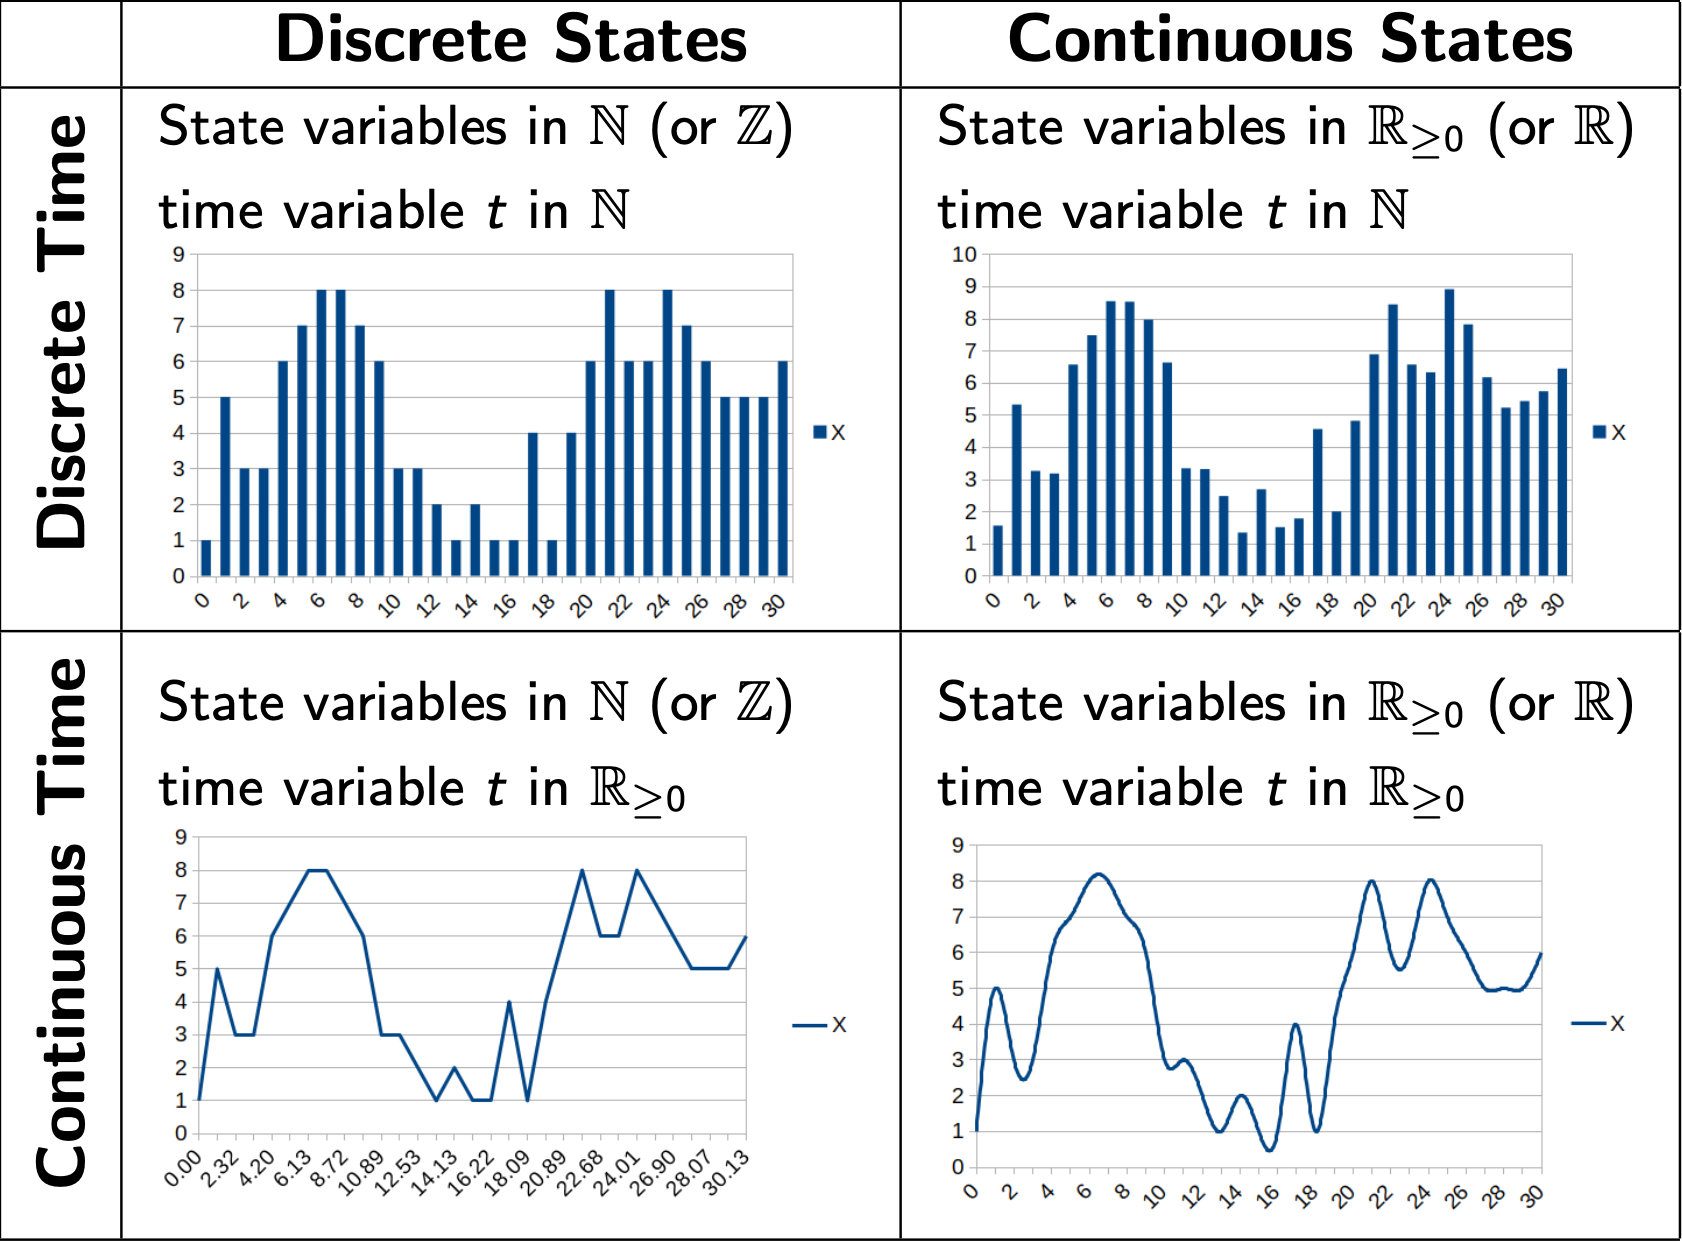
\includegraphics[width=0.8\textwidth]{Images/01-Introduction/states.png}
    \caption{All possible types of dynamical systems.}
\end{figure}

\subsection{Case of application}
What kind of analysis could we do with models of dynamical systems?

\begin{itemize}
    \item \textbf{Reachability of states:} predict the future state of the dynamical system.

    \item \textbf{Behavioral patterns:} the sequence of state that I pass through over time.

    \item \textbf{Effects of perturbations/ control strategies:} once I have a model of a system and I can simulate it, I can try to study how it will behave if I modify it.
\end{itemize}

\subsection{How to build a computational models?}
There are multiple ways

\subsubsection{The Data-driven way}
The Data-driven way (e.g. machine learning) consist in starting from the data of the system you want to model and then you apply some machine learning/optimization/whatever method to infer the model automatically. The generated model takes a form suitable for the inference method used. If enough data in available, it often works very well (good predictions), however inferred models are often very difficult to be interpreted (meaning that we can do good prediction, but we can't explain why they are correct).

\subsubsection{The Knowledge-driven way} (also called mechanistic models) consist in trying to reproduce through a mathematical model the internal mechanism of the system in order to reproduce the behaviour and to understand the internals of the systems. It requires limited data, but a good knowledge about the system functioning. Model construction usually requires some effort, and often predictions suffer from approximations but the method generated works also when few data are available; the model is interpretable: it contributes to understanding why a system behaves as observed; modelling allows validation hypotheses on the system functioning.

\section{What is a complex system?}
A complex system is a system consisting of many components (typically with a simple individual behaviours) interacting with each other, from these interaction emerges the global behaviour of the system.

\subsubsection{Complex Networks}
Complex Networks is a graph with complex structural properties. The dynamics of these networks and its evolution is a field of study (complex networks theory).

\subsection{Modeling notations for complex systems}
Many modeling languages are available for complex systems:

\begin{itemize}
    \item \textbf{mathematics:} Recurrence relations and differential equations.

    \item \textbf{concurrency theory:} we can apply methods seen in the study of concurrent system like Petri nets. Rewrite rules (Multiset rewriting) that describe the different events that happens in a complex systems as rules.

    \item \textbf{artificial life:} approaches proposed to try to reproduce behaviour seen in life. Cellular automata that describe the population as a grid; agents based model in which you explicit as an agent (e.g. an algorithm or set of functions/procedures) and then you can put the agent in a virtual environment to see how they behave together. 
\end{itemize}

\section{Analyze the model}
Modeling languages allow the modeler to express relationships between the state variables of a system and the rules/laws that determine the change of their values over time. The dynamics (or behaviour) of the systems (the actual sequences of states reached by the system over time) can be computed according to the semantics of the modeling language.

\section{Analyze the behaviour}
After the model has been specified, then there are multiple way to analyze the model. 

\subsection{Simulation}
You can try to apply some simulation algorithm in order to try to execute that model to have a possible evolution of the system. If the system is deterministic you have only one possible evolution, instead if the system is stochastic-probabilistic you will repeat the simulation several time and get different behaviour of the system. \textbf{So simulations can give you only some possible behaviour, not all}. Instead of running simulations to construct some description of the overall behaviour of the systems, it can be done by using \textbf{transition systems}. 

\subsubsection{Transition system}
A transition system is a graph (possible infinite) that describe the possible behaviour of a system. A possible transition system is the \textit{Makov chain}

\subsection{Model Checking}
It is an approach that determine whether the whole transition system satisfies a given dynamical property.

\section{Modeling vs programming}
The approach that we will follow to analyze dynamical systems is similar to the approach used to analyze programs

\begin{figure}[h]
    \centering
    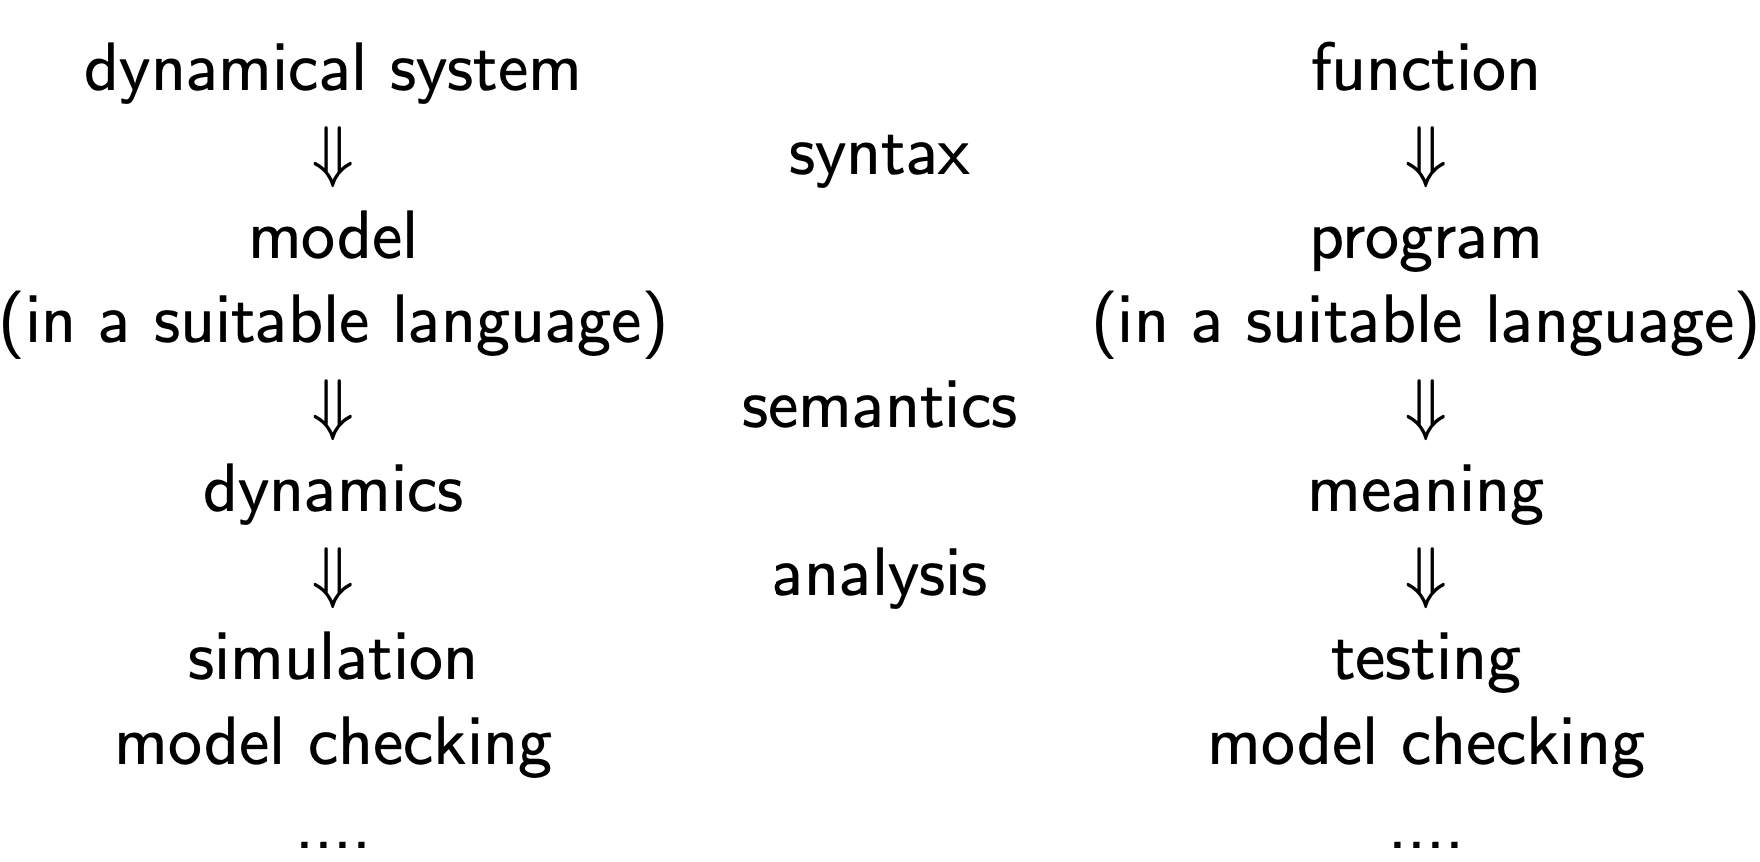
\includegraphics[width=0.9\textwidth]{Images/01-Introduction/model vs programming.png}
    \caption{Modeling vs programming.}
\end{figure}

\chapter{Discrete Dynamical Systems}
They are systems where the evolution is performed using discrete steps, in which the variables describing the state of the system are updated.

\section{Recurrence relations (Difference equations)}
Relations that tell you how from the current state of the discrete systems you obtain the next state of the systems, that is how from the original values the go to the new ones.
\par In this schema we will consider a generic system that is considered as a \textbf{population}(birth/death of individuals). Even the simplest form of interaction between individuals can lead to the emergence of \textbf{complex behaviors} (chaotic behavior) in the population. 

\section{Linear Birth Model}
The linear birth model is the simplest model describing a recurrence relation.
\par Given a population, each individual is \textbf{indistinguishable} from each other. We denote with \texttt{N(t)} the \textbf{density of some population} at a time \texttt{t}, that is the variable that describe the number of individuals that are part of the population at time \texttt{t}.
\par Given this description we want to predict what will happen to the density of the same population at a future time $t^{'} = t + \Delta{t}$ assuming that:

\begin{itemize}
    \item all individuals are indistinguishable from each other.
    
    \item there is enough food and space for every individual.
    
    \item each individual has $\lambda$ children every $\sigma$ time units.

    \item there is no death occurring in the interval $ [t, t + \Delta{t} )$.

    \item children do not start reproducing in the interval $ [t, t + \Delta{t} )$.
\end{itemize}

\begin{figure}[h]
    \centering
    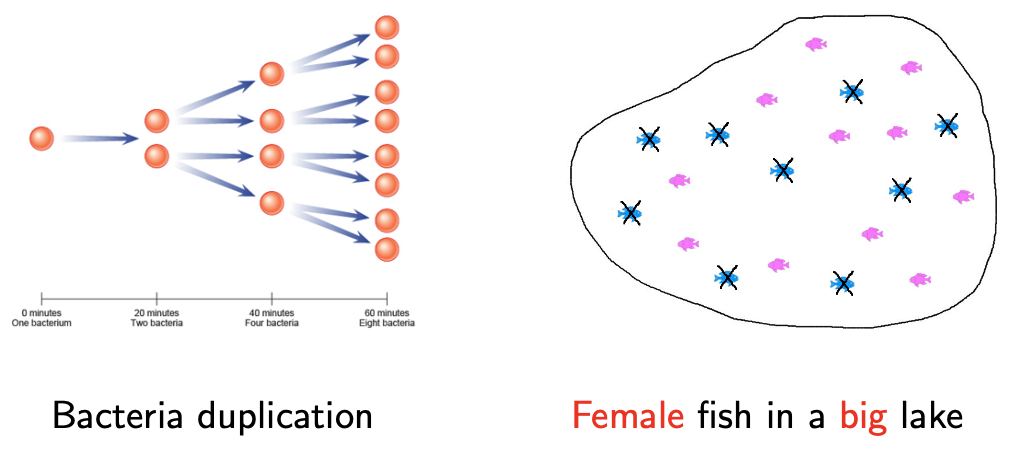
\includegraphics[width=0.8\textwidth]{Images/02-Discrete Dynamical Systems/Example_Linear_Birth_Model.png}
    \caption{Example of populations satisfying the assumption. In the bacteria example in order to assume
            the no children duplication we set $\Delta{t} \leq 20 minutes$} 
\end{figure}

\subsection{Describing the birth process as a relation}
The idea is that the size of the population at time $N(t + \Delta{t})$ will be $\geq$ than $N(t)$ since we assume \textbf{that there is no death occurring in the interval $ [t, t + \Delta{t}$]}. Additionally we know from our assumption that each \textit{adult} individual has $\lambda$ children every $\sigma$ time units.
\par Then, the number of individuals at time $t + \Delta{t}$ corresponds to the number of individuals at time $t$, plus the number of newborns at time $\Delta{t}$:

\begin{center}
    $N(t + \Delta{t}) = N(t) + \lambda{\frac{\Delta{t}}{\sigma}{N(t)}}$
\end{center}
if we group for $N(t)$ then the equation can be rewritten as follows:
\begin{center}
    $N(t + \Delta{t}) = N(t) * (1 + \lambda{\frac{\Delta{t}}{\sigma}}) $
\end{center}
    

\par Where $\frac{\Delta{t}}{\sigma}$ \textbf{describes the birth moments for every \textit{adult} individual in the interval $[t, t + \Delta{t}]$.}

\section{Constructing our algorithm}
Defined our equation \textbf{we can derive a discrete model from it}.
\par We choose a \textbf{time step} (discretization step) that describe an update of the population, in our case \textbf{the time necessary for a newborns to be considered an adult so that it can reproduce}, and we set it as $\Delta{t}$.
\par Instead of representing the equation fully we rewrite it using the \textbf{notation of sequence theory} by instead of using the actual value of the time $\Delta{t}$, we just count the steps. Thus we obtain:
\begin{center}
    $N_{t+1} = r_{d}N_{t}$
\end{center}
where $r$ stands for \textit{rate}; $d$ stands for \textit{discrete}; $r_{d}$ represents the \textbf{constant birth rate} s.t. $r_{d} = \lambda{\frac{\Delta{t}} {\sigma}}$.

\subsection{Defining the general term of our equation}
Given the recurrence relation we can \textit{sometimes} calculate the \textbf{general term}, that is the solution of the recurrence relation. In the case of our linear birth model it is a \textbf{non-recursive definition of $N_{t}$}.
\par To do so we first calculate the first terms of $N_{t}$: $N_{1}, N_{2}, N_{3}, ...$

\begin{center}
    \begin{itemize}[label={}]
        \item $N_{1} = r_{d}N_{0}$

        \item $N_{2} = r_{d}N_{1} = r^{2}_{d}N_{0}$

        \item $N_{3} = r_{d}N_{2} = r^{3}_{d}N_{0}$
    \end{itemize}
\end{center}

We notice how \textit{it seems} that $N_t = r^{t}_{d}N_{0}$, \textbf{but we have to prove it}.
To prove the formula, since we are in the realms of the natural numbers, we can use \textbf{mathematical induction}:

\begin{itemize}[label={}]
    
    \item \textbf{Base Case (t = 0):} $N_{0} = r^{0}_{d}N_{0}$ which is true.
    
    \item \textbf{Induction Case (t = k + 1):} we assume that the formula is correct for $t = 0$ to $t = k$ and check if it is true for $t = k + 1$. We know from assumption that $N_{k+1}$ will be a summation between the previous value for $t = k$ and the newborns in the current step. $N_{k+1} = r_{d}N{k}$ and we know from \textbf{induction hypothesis} that $N_{k} = r^{k}_{d}N_{0}$, thus we can rewrite $N_{k+1}$ as $N_{k+1} = r_{d}(r^{k}_{d}N_{0}) = r^{k+1}_{d}N_{0}$ proving the thesis.  
    
\end{itemize}

Now having the general term $N_{t} = r^{t}_{d}N_{0}$ we can compute the solution of our model.

\subsubsection{Phase portrait}
A way to represent recurrence relations graphically is through \textbf{phase portrait}. It consists in putting in the \textit{Cartesian plane}:
\begin{itemize}
    \item \textbf{x-axis}: $N_{t}$

    \item \textbf{y-axis}: $N_{t+1}$
\end{itemize}

Then in the plane we plot the recurrent relation. First you draw the bisector and you draw the recurrence relation as a function, then by starting from point $(N_{0}, N_{0})$ on the bisector, the other point can be obtained by \textit{"bouncing"} on the curve of the recurrence relation. \textbf{You can see how fast the quantity increases (or decreases) over time}.

\begin{figure}[h]
    \centering
    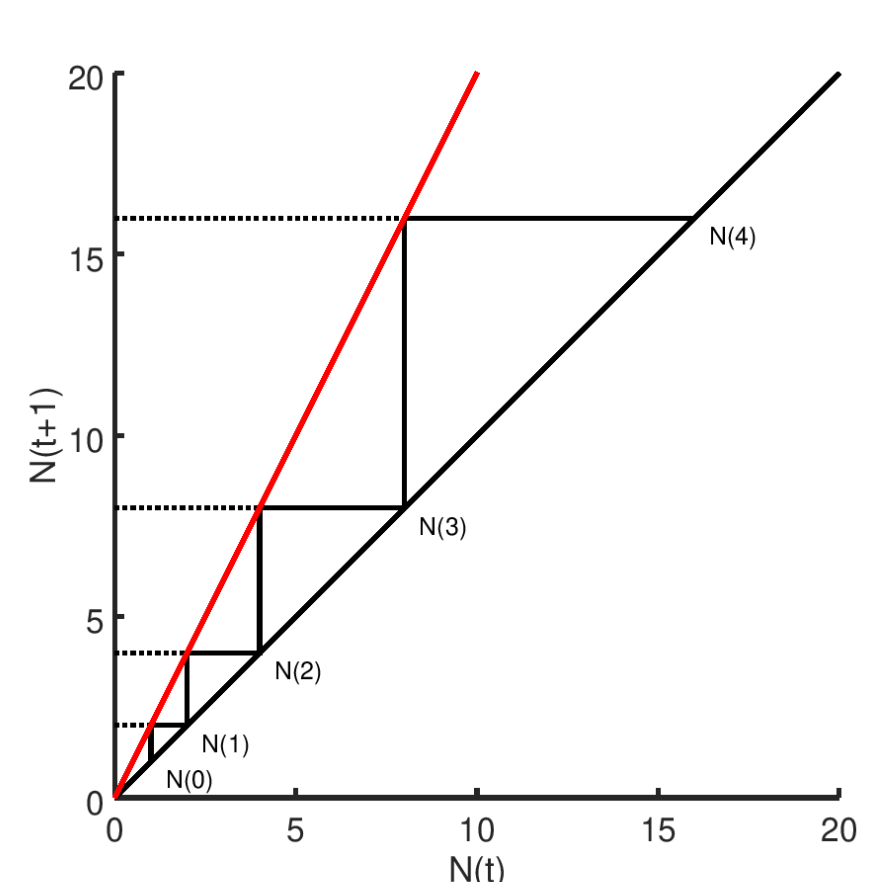
\includegraphics[width=0.5\textwidth]{Images/02-Discrete Dynamical Systems/phase_potrait.png}
    \caption{} 
\end{figure}

\begin{center}
    Above an example of phase portrait in our linear birth model. 
    \par In \textcolor{red}{red} we draw the recurrence equation $N_{t+1} = 2N_{t}$.
    in \textbf{black} the bisector $N_{t+1} = N_{t}$. 
\end{center}

\section{Introducing death in our model}
We complicate our recurrence relation by considering also deaths, so we are adding a negative term that decrease the number of individuals of our population over time. 
\par Assume that, a constant fraction $s_{d}$ \textbf{of adults that die in every time step} $\delta{t}$. Then our recurrence relation now is:
\begin{center}
    $N_{t+1} = r_{d}N_{t} - s_{d}N_{t}$
\end{center}

By grouping for $N_t$ we can rewrite the equation as:

\begin{center}
    $N_{t+1} = (r_{d} - s_{d})N_{t}$
\end{center}

\textbf{Note:} since the number of individuals which die cannot be greater than the whole population, then $ 0 \leq s_{d} \leq 1$

\par Since $r_{d}$ and $s_{d}$ are two constant, one positive and one negative, we can group them together in one single constant $\alpha_{d} = (r_{d} - s_{d})$. We call $\alpha_{d}$ the \textbf{net growth rate}, that is the rate where you discard the individuals who dies. We can rewrite our equations as:

\begin{center}
    $N_{t+1} = \alpha_{d}N_{t}$
\end{center}

The difference in respect of the previous case is that $\alpha_{d}$ will be in general greater than 0, but not necessarily greater than 1.

\subsubsection{General trend of our model}
There could be many possible cases depending on the value of the constant $\alpha_{d}$:

\begin{itemize}

    \item $\alpha_{d} > 1$: the overall behaviour of the population is the same as before, \textbf{since the population at every steps will increase}.

    \item $\alpha_{d} = 1$: the population remains constant, \textbf{since the number of newborns always is equal to the number of dead ones}.

    \item $\alpha_{d} < 1$: if for instance we assume we have less newborns than the death of old individuals, \textbf{then at every step the population reduces}.
    
\end{itemize}

\section{Introducing migration in our model}
Independently from the size of the population, \textbf{we assume a fixed number of individuals arrive in our region}. We only consider people that arrives, so we model the migration using a constant and positive parameter declared as $\beta$. 
\par Then our equation becomes:

\begin{center}
    $N_{t+1} = \alpha_{d}N_{t} + \beta$
\end{center}

with $\beta \geq 0 $ representing the number of individuals entering the population every $\Delta{t}$ time units.

\par By \textbf{mathematical induction} we can prove the general term is:

\begin{center}
    $N_{t} = \alpha^{t}_{d}N_{0} + \sum_{i=0}^{t-1}{a^{i}_{d}\beta}$
\end{center}

where $\sum_{i=0}^{t-1}{a^{i}_{d}\beta}$ accumulates the $\beta$ individuals that arrived in the previous step (from 0 to $t-1$) and the children produced by them at every step.

\subsection{Simulating the migration}
Having our general term, we can see what happens by varying $\alpha_{d}, N_{0}$ and $ \beta:$
\par \textbf{Case $\alpha_{d} > 1$}

\begin{figure}[h]
    \centering
    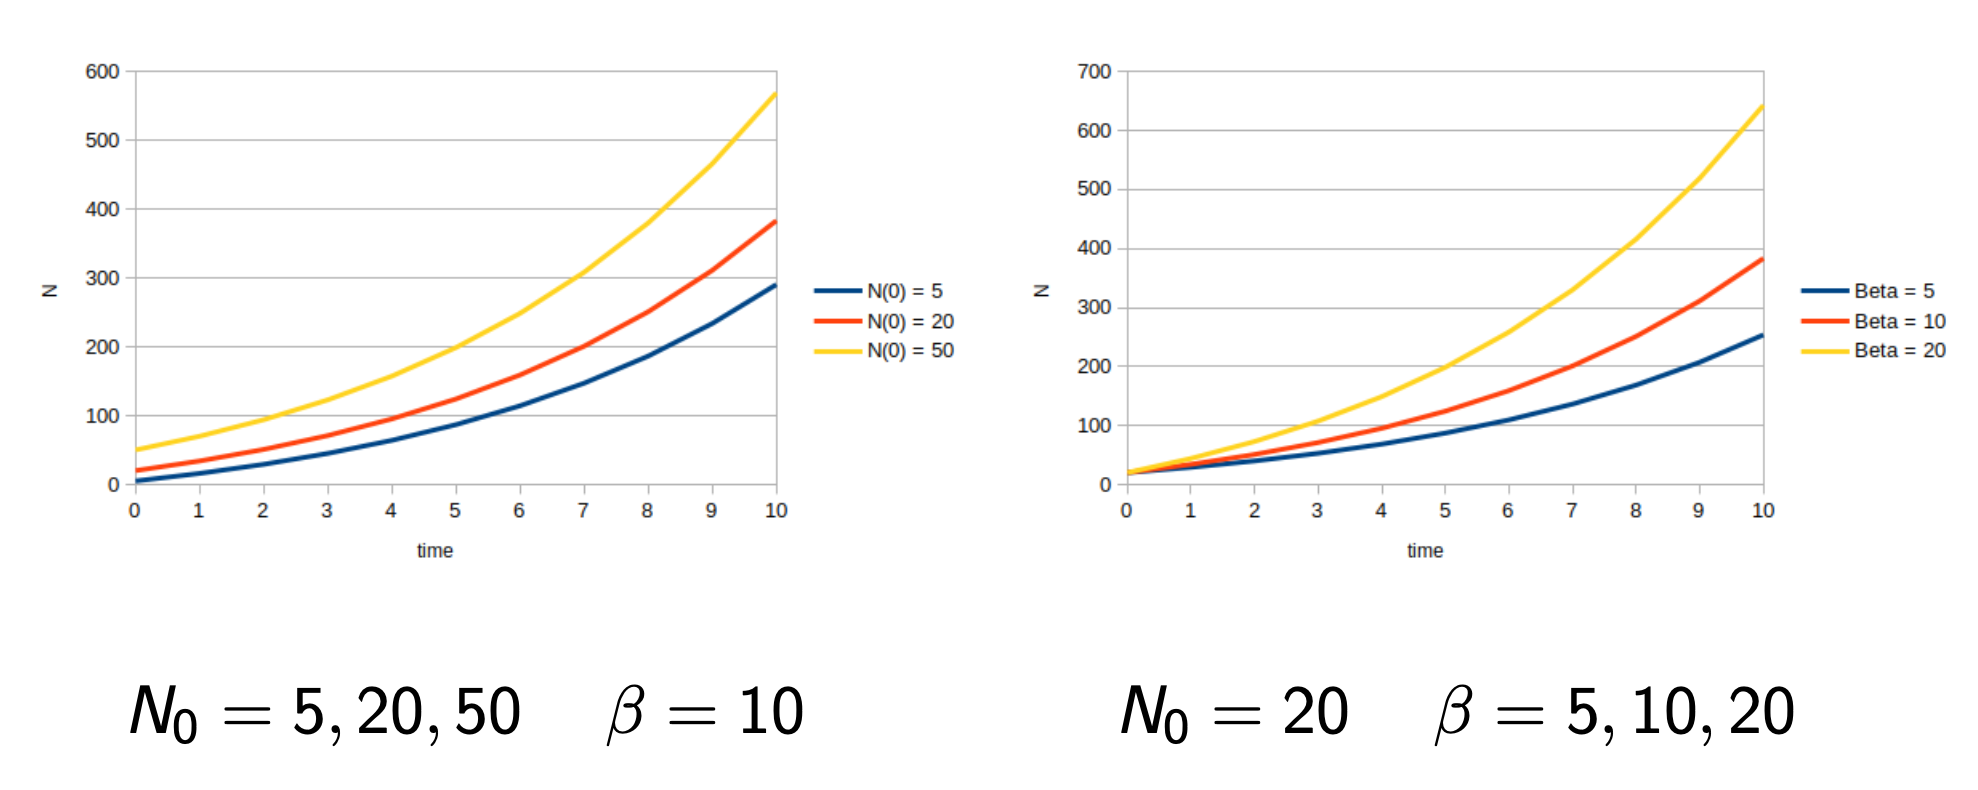
\includegraphics[width=0.9\textwidth]{Images/02-Discrete Dynamical Systems/case_1.png}
    \caption{The dynamics is dominated by the birth process (exponential growth).} 
\end{figure}

\par \textbf{Case $\alpha_{d} = 1$}

\begin{figure}[h]
    \centering
    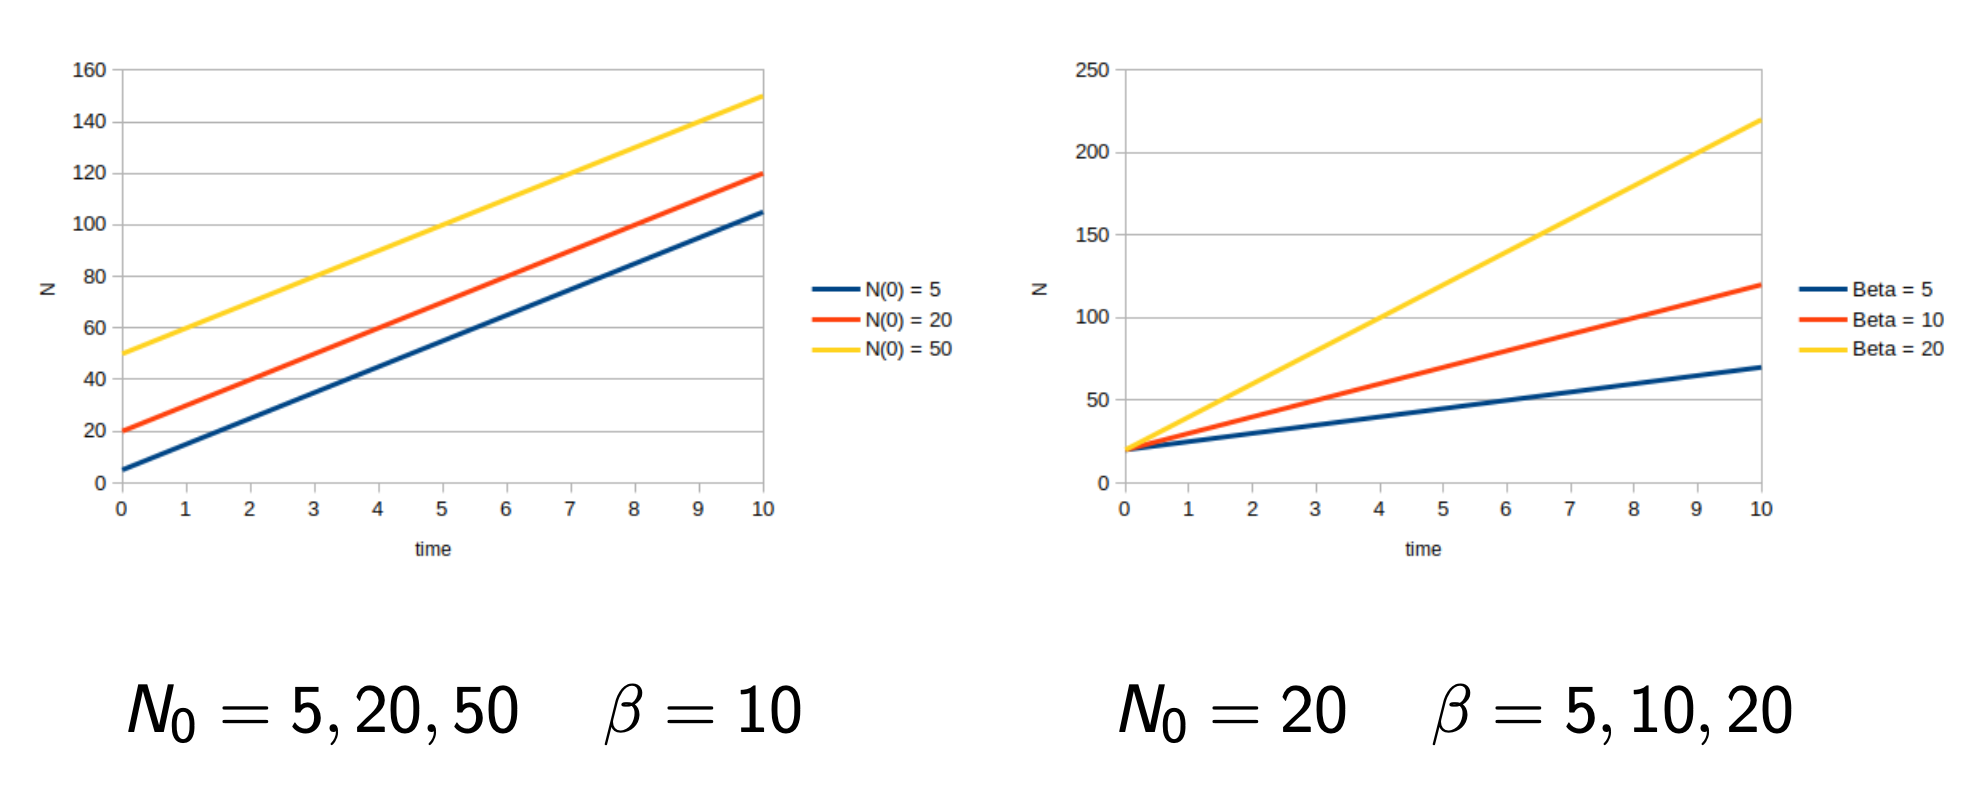
\includegraphics[width=0.9\textwidth]{Images/02-Discrete Dynamical Systems/case_2.png}
    \caption{The dynamics is dominated by the migration process (linear growth).} 
\end{figure}

\par \textbf{Case $\alpha_{d} < 1$}

\begin{figure}[h]
    \centering
    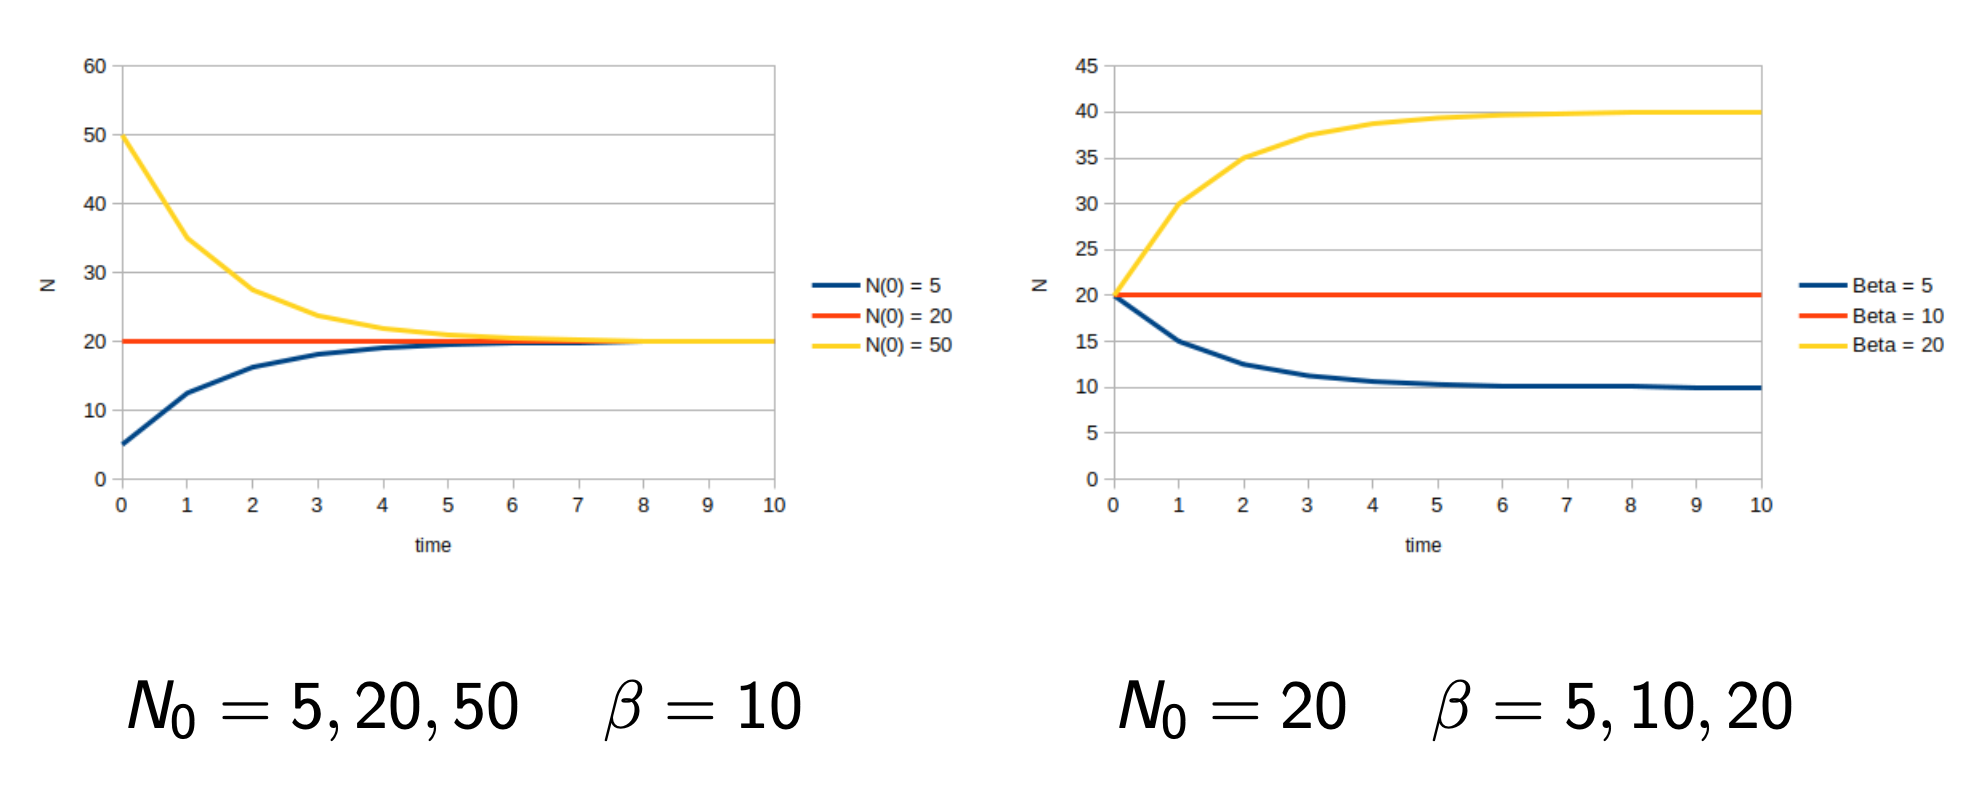
\includegraphics[width=0.9\textwidth]{Images/02-Discrete Dynamical Systems/case_3.png}
    \caption{The population reaches a dynamic equilibrium: a stable state in which opposite phenomena compensate each other (migration compensates deaths). Note that it is independent from $N_{0}$} 
\end{figure}

\subsection{Computing the equilibrium point}
The equilibrium point (also called saturation point) is defined as the moment $t=k+1$ where the computed size of the population is the same as the previous step, that is:

\begin{center}
    $N_{t-1} = N_{t}$
\end{center}

Knowing that $N_{t} = \alpha_{d}N_{t} + \beta$ we solve the equation in regards to $N_{t}$ and obtain:

\begin{center}
    $N_{t} = \frac{\beta}{1 - \alpha_{d}}$
\end{center}

\subsection{Non-linear models}
So far we have described a population where each individual behaves autonomously, which do not fit the definition of complex system (many components with very simple individual behaviour \textbf{that interact with each other and the environment}). Introducing interaction between the individuals \textbf{requires a non-linear model} (previously we used a linear one). In our (Non-linear) Birth Model now the environment has limited resources such as food and place, thus requiring that the individuals compete \textbf{(a form in interaction)} for survival.

\section{Rewriting our equation}
For simplicity assume we are in a closed environment (no migration), then we define $K$ as the \textbf{carrying capacity of the environment}, meaning that in the environment there is enough food and space for $K$ individuals.
\par The population is still governed by the birth rate, but now death is no more a constant, instead is negatively influenced by $K$:

\begin{center}
    $N_{t+1} = r_{d}N_{t}(1 - \frac{N_{t}}{K})$
\end{center}
\textbf{Note:} this non-linear equation is called \textbf{logistic equation} (it is an alternative formulation)

So now the birth rate is modulated by the ratio of occupancy on the environment $\frac{N_{t}}{K}$:

\begin{itemize}

    \item $N_{t}$ close to 0 : we have a simple birth process with rate $r_{d}$ (exponential growth). 

    \item $N_{t}$ increases: the growth tends to stop.

\end{itemize}

Eventually the population reaches a \textbf{dynamic equilibrium} representing the situation in which environment resources are fully exploited (\textbf{saturation})

\begin{figure}[h]
    \centering
    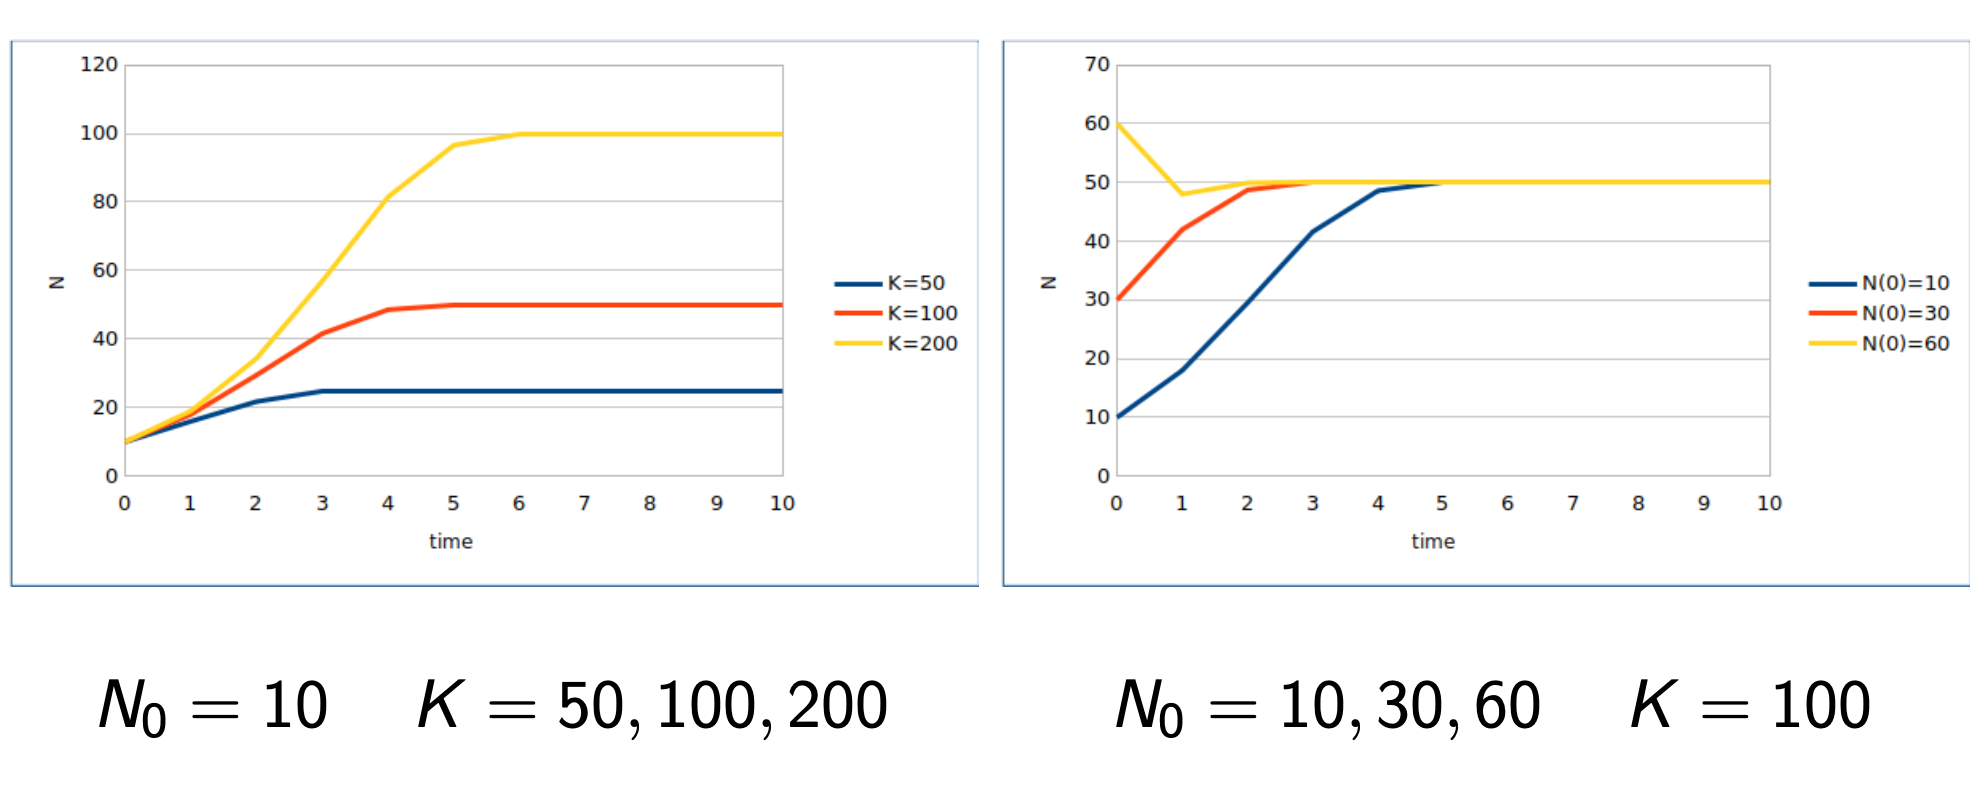
\includegraphics[width=0.9\textwidth]{Images/02-Discrete Dynamical Systems/Non-linear .png}
    \caption{The first graph shows a case where the equilibrium point depends on $K$. The second graph shows me that the equilibrium point is independent from the initial number of individuals.} 
\end{figure}

\section{Removing homogeneity}
For now we have considered an homogeneous population, but in realistic case we have different individuals with different features and we want to consider each group of individuals. In the system point of view this requires not just a single recurrence equation, but a \textbf{system of recurrence equations}. 
\par consider a population of fishes that live in a pond. Each individual can either be a male fish, modelled as $M_t$ or a female fish, modelled as $F_t$. We consider that a small part of males dies because of fights among them (death rate $s_d$).
\par then we construct a system of recurrence equations:


\[
\begin{cases}
    \begin{aligned}
        F_{t+1} = r_{d}F_{t}(1 - \frac{F_{t} + M_{t}} {K}) \\
        M_{t+1} = r_{d}F_{t}(1 - \frac{F_{t} + M_{t}}{K}) - s_{d}M_{t}\\
    \end{aligned}
\end{cases}
\]

where:
\begin{itemize}
    \item $r_{d}F_{t}$ represent the number of child born, note that they are generated by females.

    \item $F_{t} + M_{t}$ describes the whole population size (to be related with the carrying capacity K).
\end{itemize}

\section{Limitation of discrete dynamical models}
Discretization of the system dynamics may introduce inaccuracies: recurrence equations assume that nothing happens during the $\Delta{t}$ time that occurs between $N_{t}$ and $N_{t+1}$. Adjusting $\Delta{t}$ to be smaller usually correspond to more accurate approximations, more precisely we should let $\Delta{t}$ tend to 0.


\chapter{Continuous Dynamical Systems}

\section {Recap - Why we need to introduce ODEs}
As we said in the previous chapter, using a discrete representation for the steps in our model can lead us to lose all the informations that happens between the step $N_t$ and the step $N_t+1$. \par
The simplest solution is to make the distance in time $\Delta t$ between the to step very small ($\approx 0$), but it is not enough.

\section{Reconsidering the population model}
Recall in our population model that with $N(t)$ we denote the \textbf{density of some population} at time t. Our goal is to construct a mathematical model able to predict the density of the same population at a time $t^{'} = t + \Delta{t}$.

\subsection {Introducing the Ordinary Differential Equation}

\par Given our equation which is based the model:
\begin{center}
    $N(t + \Delta{t}) = N(t) + \lambda{\frac{\Delta{t}}{\sigma}{N(t)}}$
\end{center}
And the corresponding \textbf{recurrence equation}:
\begin{center}
    $N_{t+1} = r_{d}N_{t}$
\end{center}
where $r_{d} = \frac{\Delta{t}}{\sigma}$ consider the case where $\Delta{t} \rightarrow 0$. This case cannot be done using discretization, because it can lead to inaccuracies.
\par To handle the case $\Delta{t} \rightarrow 0$ we make some transformation to our equation:

\begin{center}
    $N(t + \Delta{t}) = N(t) + \lambda{\frac{\Delta{t}}{\sigma}{N(t)}} \rightarrow  \frac{N(t + \Delta{t}) - N(t)}{\Delta{t}} $
\end{center}

then by simplifying we get:

\begin{center}
    $ \frac{N(t + \Delta{t}) - N(t)}{\Delta{t}} = \frac{\lambda}{\sigma}N(t) $
\end{center}

We can recognize that the left hand side can be traced back as the \textbf{difference quotient} $\frac{f(x + h) - f(x)}{h}$, \textbf{which when taken to the limit as h approaches 0 gives the derivative of the function f}.
\par Let's consider our equation for $\Delta{t} \rightarrow 0$:

\begin{center}
    $\lim_{\Delta{t} \to 0} \frac{N(t + \Delta{t}) - N(t)}{\Delta{t}} 
    = 
    \lim_{\Delta{t} \to 0} r_{c}N(t)$
\end{center}

with $r_{c} = \frac{\lambda}{\sigma}$

Note that on the right hand side $\Delta{t}$ doesn't appear, thus we can remove the limit; the term on the left hand side is the derivative of $N(t)$, indicated as simply $\dot{N}(t)$. Thus we simply the equation as follows:

\begin{center}
    $\dot{N}(t) = r_{c}N(t)$
\end{center}

We have defined the dynamics of the system as the derivative equal to a constant multiplied by the value of the function at time $t$.\par \textbf{This equation is known as Ordinary Differential Equation (ODE)}.
\par An ODE has the following properties:
\begin{itemize}
    \item it relates the function $N$ with its derivative $\dot{N}$

    \item $t \in \mathbb{R}$, \textbf{so time is continuous}
\end{itemize}

\par We would like to use the Ordinary Differential Equation to run some simulation or to compute a general solution (like we did for the recurrence relation). 

\subsection{Using the ODE}
In some very simple case, like our linear birth model, we can find the general solution by finding a closed-form definition of $N(t)$ satisfying the equation. \textbf{A closed-form definition is one that depends only on t and some constant}. 
\par for the linear growth model a solution can be found analytically. 

\par Recall our equation:
\begin{center}
    $\dot{N}(t) = r_{c}N(t)$
\end{center}
Now let's move $N(t)$ from the right to the left hand-side of the equation:

\begin{center}
    $\frac{\dot{N}(t)}{N(t)} = r_{c}$
\end{center}
Recall that $\frac{\dot{N}(t)}{N(t)} = \ln{N(t)}$ and $r_{c}$ is the derivative of $r_{c}t + c$ for any constant $c$, obtaining:

\begin{center}
    $\ln{N(t)} = r_{c}t + c$
\end{center}
By resolving our equation in regards to $N(t)$ we finally get:
\begin{center}
    ${N(t)} = Ce^{r_{c}t + c}$
\end{center}
where $C = e^{c}$ (typically $C$ is set to be equal to $N(0)$

\begin{figure}[h]
    \centering
    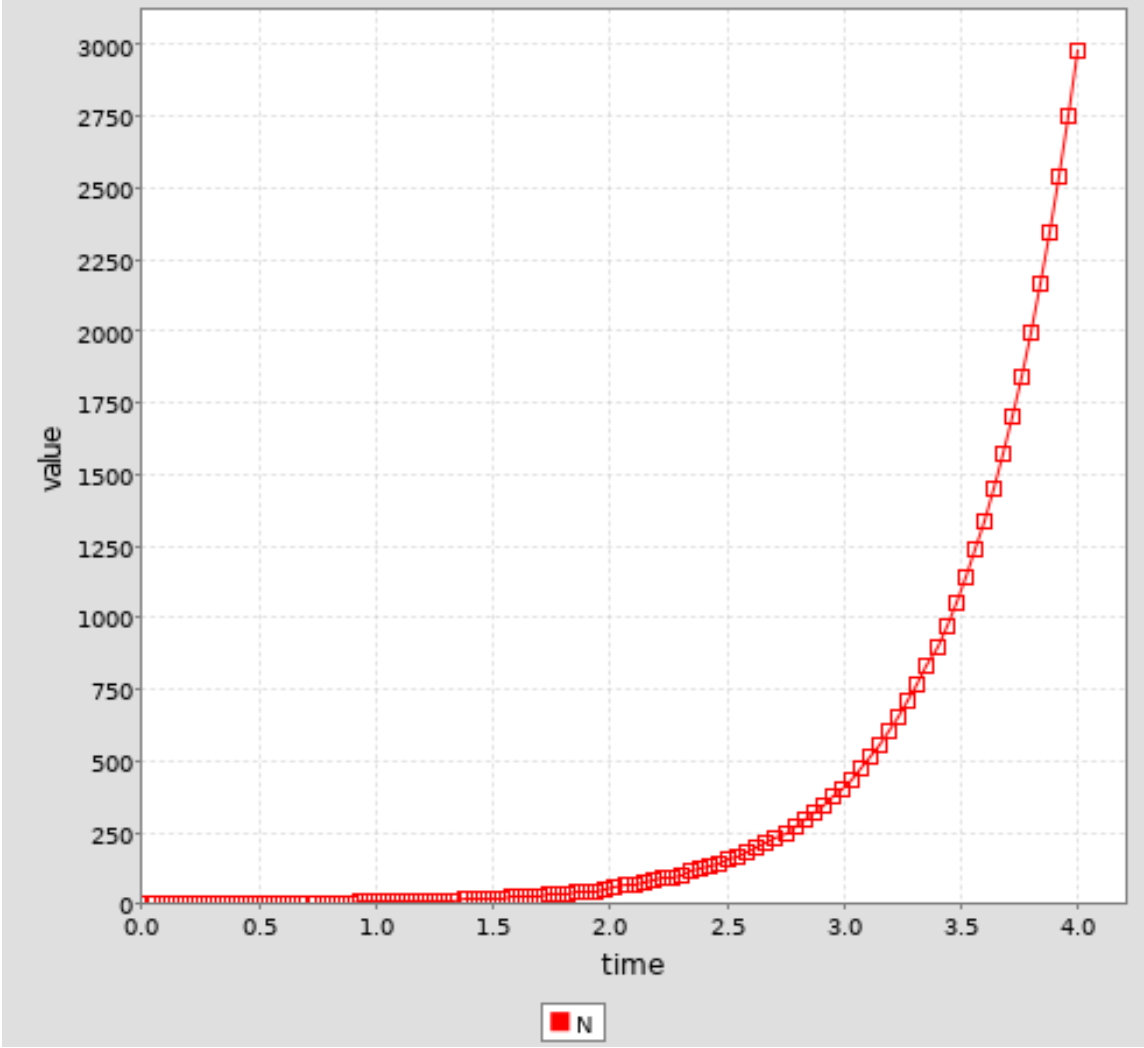
\includegraphics[width=0.5\textwidth]{Images/03 - Contiguous Dynamicsl System/linear_birth_model_continuous.png}
    \caption{This graphs shows us that by setting in our population model $r_{c} = 2$ and $C = N(0) = 1$ then the population shows an exponential growth over time.} 
\end{figure}

\subsubsection{Differences between discrete and continuous model}
This behaviour is qualitatively the same as for the discrete model, both showing exponential growth.
\textbf{What changes is the meaning of the equation}: 
\begin{itemize}
    \item the recurrence relation tells you how to update the variable.

    \item in our new equation it defines the derivative, \textbf{meaning how fast it's changing}.
\end{itemize}
Note how both equations show rate $\geq 1$ only if the birth rate $\frac{\lambda}{\sigma}$ is $\geq 1$.

\section{Example - Radioactive decay}
We move from the example of the population model we have seen so far to another one.
\par Radioactive decay is a process where we have a negative evolution of the population. The idea is that \textbf{each molecule decays at a constant rate}, so the whole mass decreases with a rate which is proportional to the mass itself.
\par We can describe this model by using the following Ordinary Differential Equation:

\begin{center}
    $\dot{N}(t) = -d_{c}N(t)$
\end{center}
then if we solve it in regards to $N(t)$ we get:
\begin{center}
    $N(t) = N(0)e^{-d_{c}t}$
\end{center}

\begin{figure}[h]
    \centering
    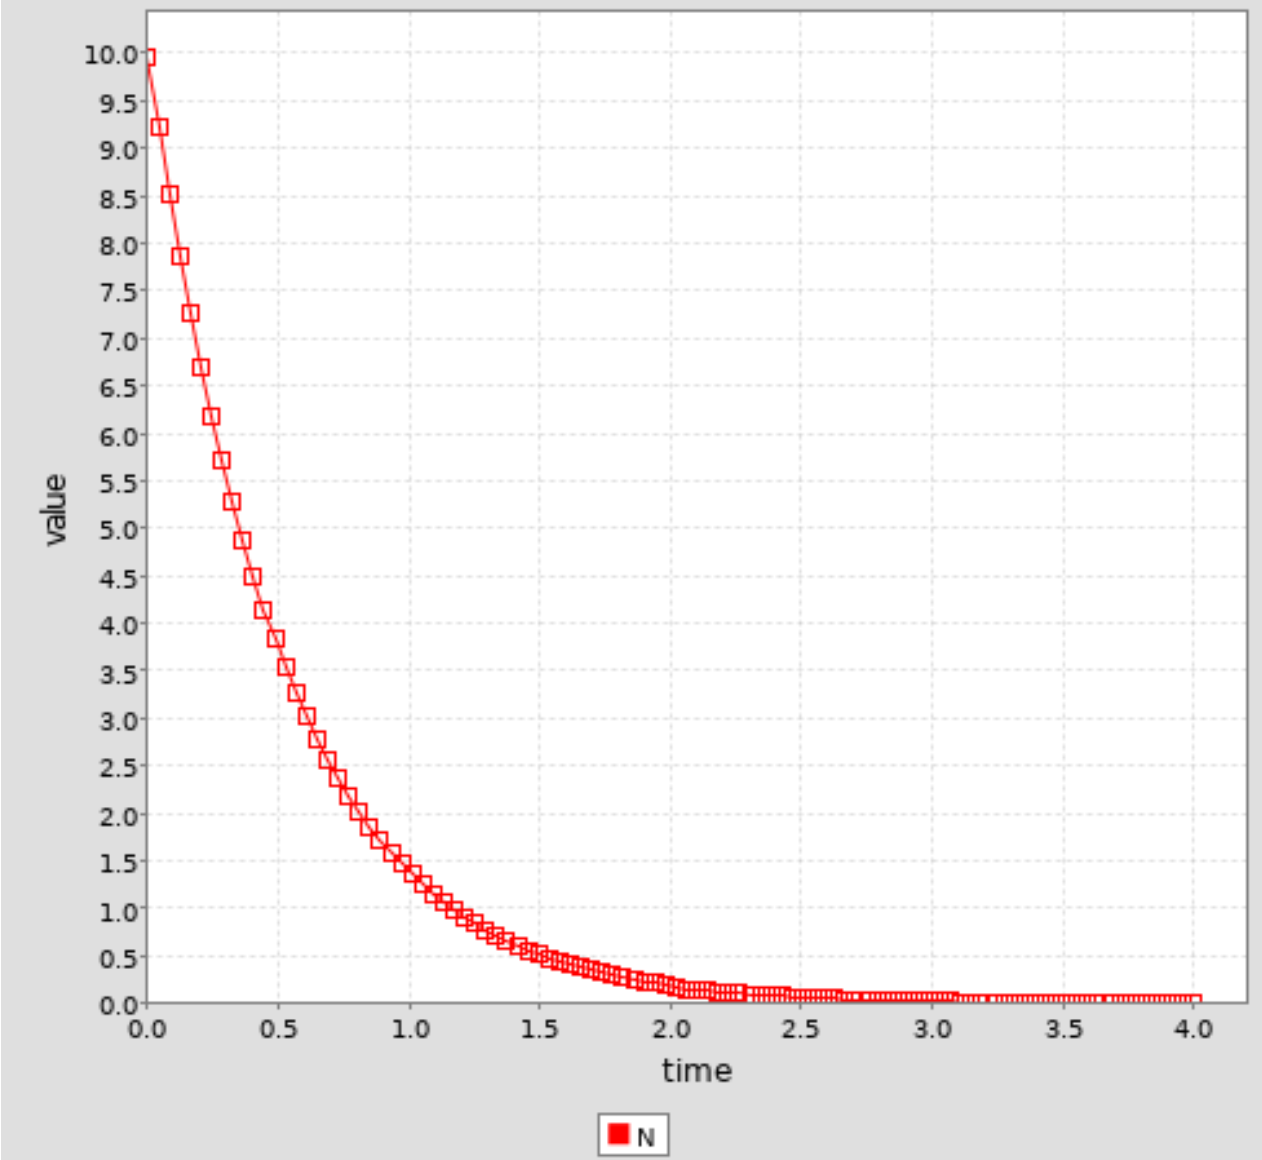
\includegraphics[width=0.5\textwidth]{Images/03 - Contiguous Dynamicsl System/Radioactive_decay.png}
    \caption{Example of applying the ODE of the radioactive decay. Note that  by setting $d_{c} = 2$ and $C = N(0) = 10$ we get $N(t)$ to tend to zero. This is caused by the negative exponent in the ODE.} 
\end{figure}

\section{Continuous version of the logistic equation}
Given the non-linear logistic equation, we can define as follows its continuous version:
\begin{center}
    $\dot{N}(t) = r_{c}N(t)(1 - \frac{N(t)}{K})$
\end{center}
where:
\begin{itemize}
    \item $r_{c}$ is the \textbf{continuous growth rate}.

    \item $K$ is the \textbf{carrying capacity} of the environment.
\end{itemize}

Resolving the ODE in regards to $N(t)$ we get:
\begin{center}
    $N(t) = \frac{K}{1 + (\frac{K}{N(0)} - 1) e^{-r_{c}t}}$
\end{center}
We notice that when $N(t) \rightarrow K$ \textbf{the population converges to the carrying capacity of the environment}.

\begin{figure}[h]
    \centering
    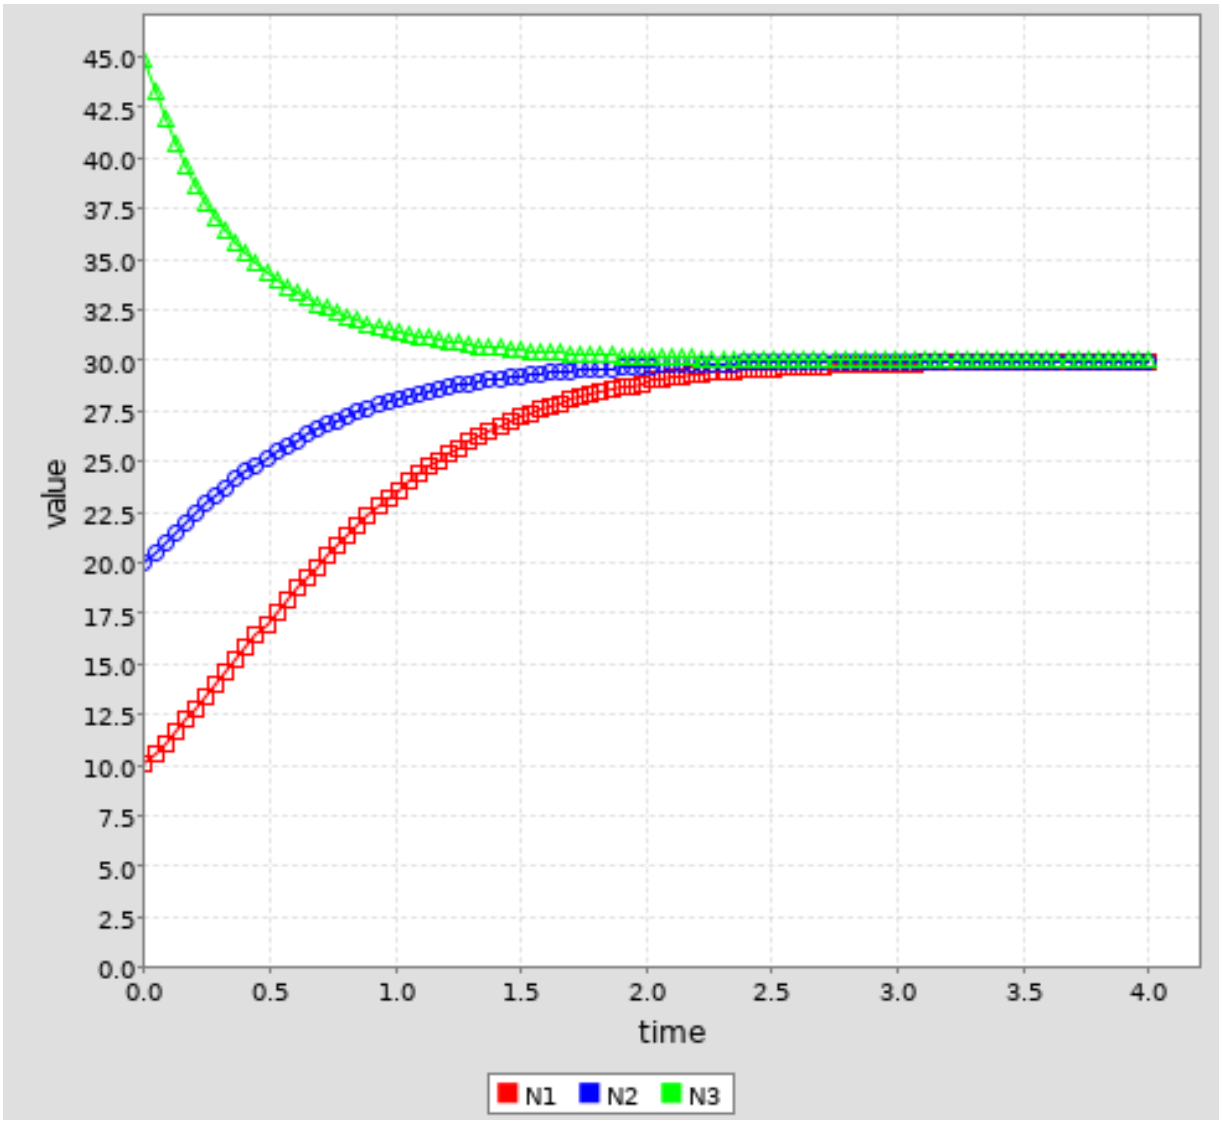
\includegraphics[width=0.5\textwidth]{Images/03 - Contiguous Dynamicsl System/continuous_logistics.png}
    \caption{Example of the continuous logistic equation. Note how by putting $r_{c} = 2$, $N(0) = 10$, $K = 30$, the population will eventually converge to the carrying capacity of the environment.} 
\end{figure}

\par \textbf{The trend is the same as for the discrete case}.

\section{Systems of ODE}
Now let's consider a population of males, indicated as $M(t)$, and females, indicated as $F(t)$. Assume that males fight with each other, so a small part of them dies because of it with a death rate of $s_{c}$. 
\par Thus we have to expand our model considering a system of ODEs:
\[
\begin{cases}
    \begin{aligned}
        \dot{F}_{t} = r_{c}F_{t}(1 - \frac{F_{t} + M_{t}} {K}) \\
        \dot{M}_{t} = r_{c}F_{t}(1 - \frac{F_{t} + M_{t}}{K}) - s_{c}M_{t}\\
    \end{aligned}
\end{cases}
\]
where:
\begin{itemize}
    \item $r_{c}F(t)$ is used for both genders, \textbf{since both are generated by females}.
    \item $F(t) + M(t)$ describes the whole population size.
\end{itemize}

\begin{figure}[h]
    \centering
    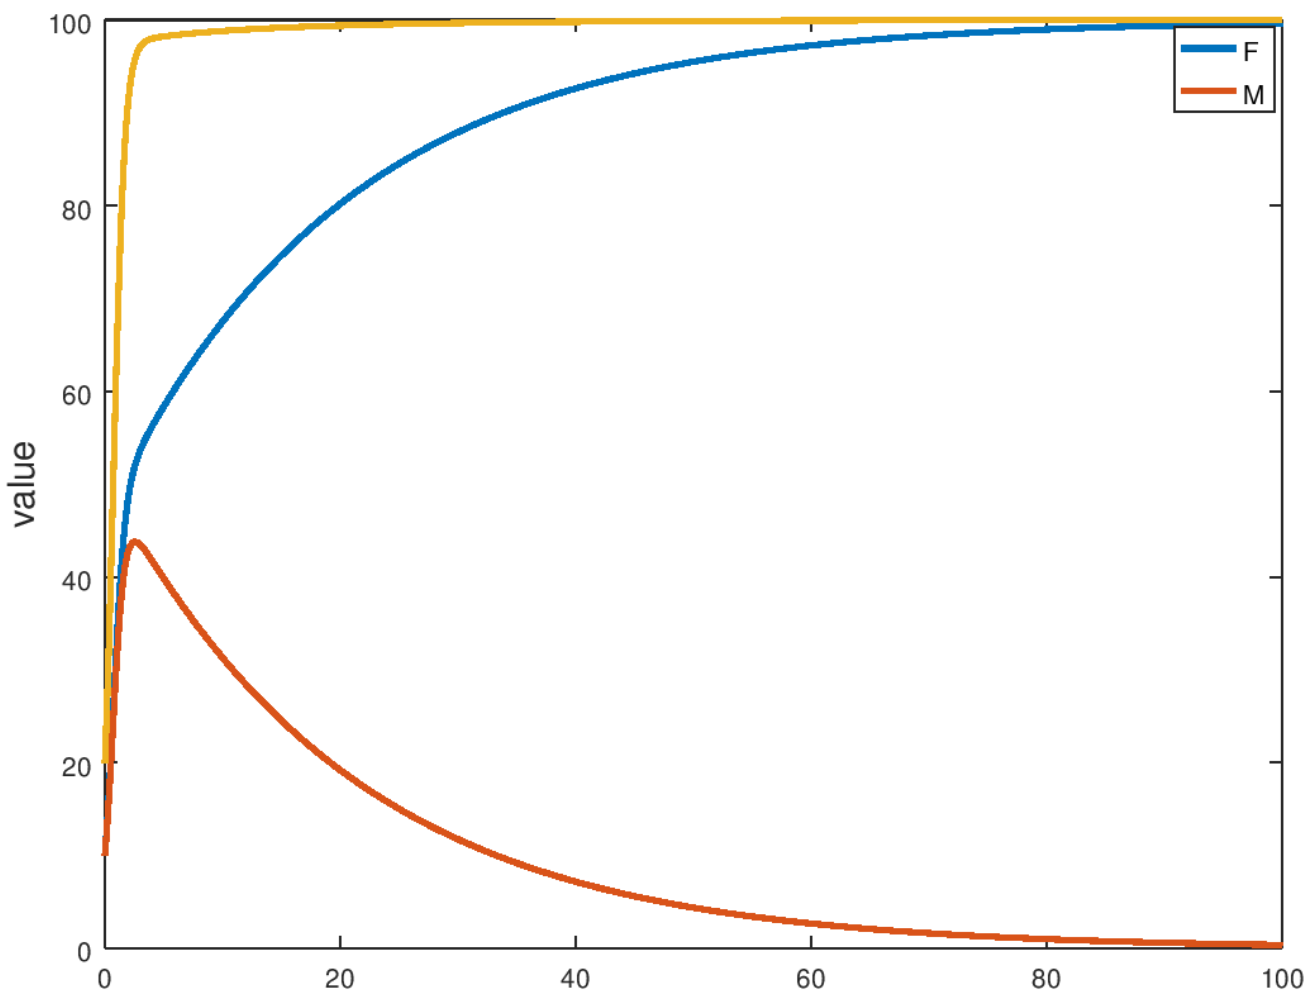
\includegraphics[width=0.5\textwidth]{Images/03 - Contiguous Dynamicsl System/system of ODE.png}
    \caption{Example of the system of ODEs.} 
\end{figure}

What happens in this scenario, after some times you have only females in the population. This shows a completely different behaviour from the discrete case, \textbf{because the meaning of their equations is different}:
\begin{itemize}
    \item The recurrence relations indicates us the size of the population.

    \item The system of ODEs describes how fast is changing.
\end{itemize}

\section{Numerical Solution of ODEs}
Recall that we said that computing the solution of an ODE is not always possible. For this reason we prefer working using an approximation of the solution, indicated as \textbf{numerical solver} (or numerical simulator). This approximation doesn't compute the general function, \textbf{instead it solves the initial value problem, also called Cauchy problem}.

\begin{center}
\subsubsection{Initial Value Problem}
Given an ODE in the form $\dot{N}(t) = f(N(t)) $ and an initial value $N_{0}$ s.t. $N(0) = N_{0}$, compute a function $F(t)$ that is a solution of the ODE and s.t. $F(0) = N_{0}$.
\end{center}

In our case we are interested only in studying the values of $F(t)$ where $t \geq 0$, \textbf{hence we perform a numerical simulation starting at} $t = 0$.

\section{The Euler method}
The Euler method is the simplest numerical simulation method available. The main concept behind this approach is to approximate the given continuous system with a recurrence relation specifically designed to approximate the continuous differential equation. \textbf{The idea is that, since we know the derivative, we use it as it was the function}.\par
It is based on the idea of discretizing the dynamics of differential equations by time steps of constant length $\tau = \Delta t$.\par
Given an Ordinary Differential Equation in the form:

\begin{center}
$\dot{N}(t) = f(N(t))$ 
\end{center}
this corresponds to approximating its solution with the following recurrence relation (assuming $N_0 = N(0)$) 
\begin{center}
$N_{k+1} = N_k + \tau f(N_k)$ 
\end{center}
where $N_k \approx N(\tau k)$

\begin{figure}[h]
    \centering
    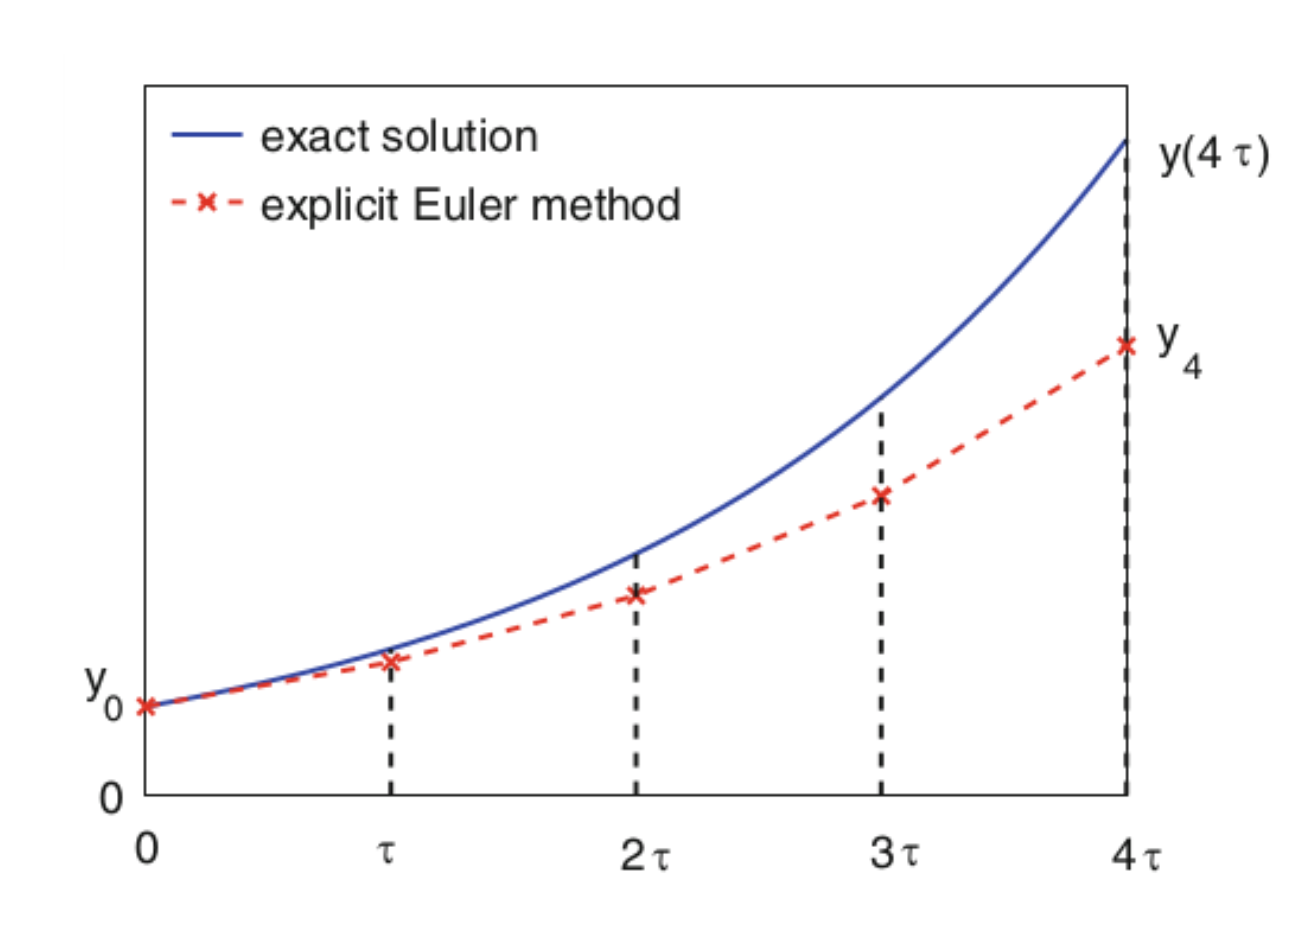
\includegraphics[width=0.5\textwidth]{Images/03 - Contiguous Dynamicsl System/Euler_method.png}
    \caption{A graph showing the correct solution compared to the approximation generated by the Euler method.} 
\end{figure}

\subsection{Errors in the Euler method}
By approximating in each step the Euler method makes local errors that will contribute to a global error at the end of the whole simulation.\par

\textbf{The local discretization error} is computed as $| N(\tau) - N_1|$ and it is in the order of $O(\tau^2)$ \textit{(the motivation is because we truncate the Taylor Series at the first step)}.\par

\textbf{The Global discretization error} is obtained by accumulate all the local discretization errors after $k$ steps, namely at time $t = k \tau$. The global error is computes as $|N(k \tau) - N_k)$ and is in the order $O(k \tau^2) = O(\tau)$ since $k \tau = t$ is constant.

\section {Other numerical simulation methods}
A linear error of $O(\tau))$ is quite annoying, requiring us to set $\tau \approx 0$ in order to have something acceptable, making the computation very slow (it requires a lot of steps).\par
To overcome this other methods have been proposed, having a global discretization error of a higher order (e.g. $O(\tau^p)$ for some p) which is better as long as $\tau \rightarrow 0$ (hence $\tau < 1$). To work these method use more than one point to approximate the value of the function, making a single step require more time, but maintain the error inside some defined boundaries. \par

A few examples of such methods are:
\begin{itemize}
    \item \textbf{Runge-Kutta methods:} $p = 2$ in the original formulation, but can be higher
    \item \textbf{Multistep methods (e.g. Adams methods):} extrapolate the value of the next step from the values of the previous k steps obtaining $p \approx k$.
\end{itemize}

State-of-art methods can also:
\begin{itemize}
    \item \textbf self-determine the step size $\tau$ based on thresholds on local and global discretization errors.
    \item \textbf dynamically adjust the step size $\tau$ during their executing (e.g. Adaptive Runge-Kutta) 
\end{itemize}

\section{Instability and stiff systems}
There is another problem that could arise: if you have a derivative which cause the value of a variable in a very fast way, if $\tau$ is not small enough you not only pay some error but you could have that your computed solution is unstable.\par
What we mean for unstable is that we lose informations and your points start to oscillate creating chaos.\par

\begin{figure}[h]
    \centering
    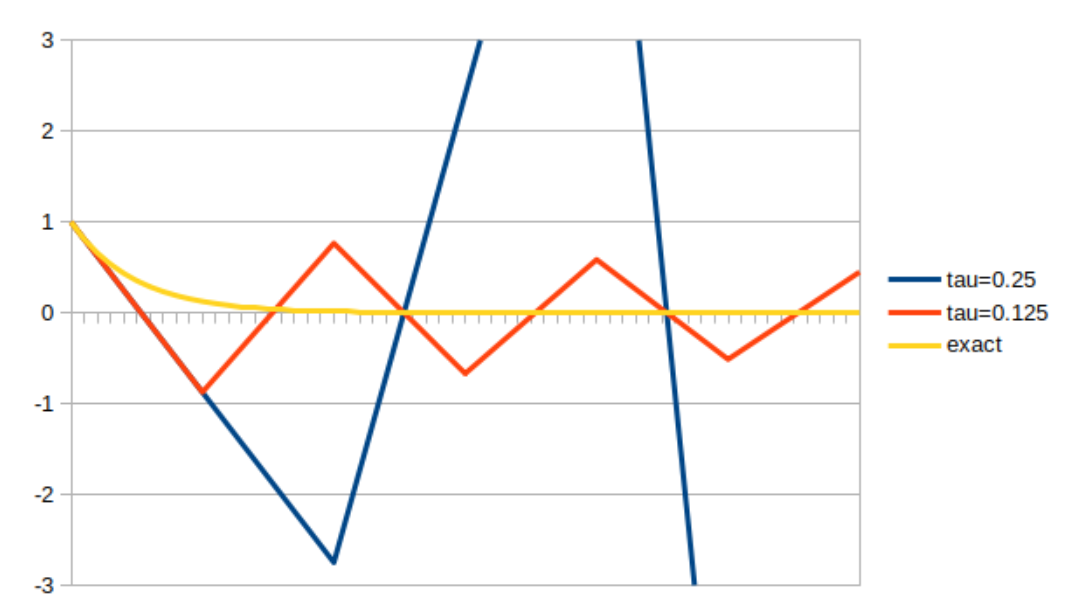
\includegraphics[width=0.5\textwidth]{Images/03 - Contiguous Dynamicsl System/Stiff System.png}
    \caption{An example of a stiff system. In orange is shown the real solution, while in red and blue the one obtained by setting $\tau$ to different values} 
\end{figure}

This kind of problematic systems are called \textbf{stiff systems}. There is no clear definition of stiffness: intuitively contains a very fast term that cannot be captured by our method, worse if we have in our systems also slow terms to take into account. \par
In this cases you need to consider alternative numerical simulation methods called \textbf{implicit numerical simulation methods}. All the methods we have seen so far have and implicit version, which requires more computation time for step.

\section{Implicit Euler method}
The idea of the implicit version of the Euler method is that, like the previous version we approximate the function by using its derivative, \textbf{but the derivative is not computed on the value $N$ at step $k$, but at the step $k+1$}.\par
By using this approach we are no longer defining $N_{k+1}$ in terms of $N_k$, but as an equation where $N_{k+1}$ is in both sides:

\begin{center}
    $N_{k+1} = N_{k} + \tau f (N_{k+1})$
\end{center}
where $N_k \approx N(k \tau)$.\par

There are methods from numerical analysis that are able to solve these type of equations. This method requires more effort for computing a single step, but \textbf{often} the local discretization error is smaller permitting us to use greater values of $\tau$.

\section{Other implicit methods}
Implementations of implicit methods that use more than one variables require the modeler to provide the \textbf{Jacobian matrix} (partial derivatives) of the function f. Most are able to compute the Jacobian matrix autonomously by doing some approximation. \par
There exist methods that are able to automatically switch from explicit to implicit methods by determining if the system is stiff.








\nocite{*}
\bibliographystyle{plain}
\clearpage\bibliography{bibliography}

\end{document}